\chapter{Implementierung}
\label{Kap5}
Die zuvor herausgearbeiteten Konzepte werden nun im bereits vorhandenem Webportal umgesetzt. Dabei wird der bisherige Aufbau der Anwendung analysiert und erweitert. Einzelne wichtige Aspekte werden in diesem Kapitel herausgegriffen und erläutert.

\section{Offline Metadaten}
Jeder Inhalt auf CROSSLOAD besitzt Eigenschaften, die hier als Inhalt oder Metadaten bezeichnet werden. Dazu gehören zum Beispiel die id, Titel, Bibelstellen, Ort oder Datum. Diese Daten werden benötigt, um Suchergebnisse oder die Detailseite einer Predigt anzuzeigen. In diesem Kapitel werden Strategien beschrieben wie diese Inhalte gecached werden, um eine bestmögliche Nutzererfahrung zu bieten.

\subsection{Detailseite}
Im Webportal CROSSLOAD wird bereits ein Service Worker verwendet, der einerseits statische Inhalte zwischenspeicher aber auch dynamische Requests cached. Für dynamische Request wurde bislang die Cache Strategy freshness verwendet. Das heißt, dass der Cache nur verwendet wird wenn der Netzwerk-Request fehlschlägt \autocite{angular-service-worker}. Angular Service Worker unterstützten noch eine zweite Cache Strategie, die immer den Wert aus dem Cache zurück gibt wenn er verfügbar ist \autocite{angular-service-worker}. Die momentane Lösung ist nicht optimal. Sie ermöglicht zwar eine Offlineverfügbarkeit der Daten aber bietet nicht die optimale Geschindigkeit für den Nutzer. In vielen Fällen wird sich der Inhalt im Cache nicht mit der Anwort aus der Netzwerkanfrage unterscheiden, trotzdem muss der Nutzer auf die Antwort vom Netzwerk warten. Eine bessere Lösung ist folgende:

Wenn der Nutzer einen Inhalt möchte, wird direkt im Cache nachgeschaut ob der Inhalt existiert. Wenn er existiert wird er dem Nutzer angezeigt. Gleichzeitig wird eine Netzwerkanfrage geschickt. Sobald die Antwort vom Netzwerk da ist wird die Antwort mit dem Wert im Cache verglichen. Wenn sich die Werte unterscheiden wird der Cache aktualisiert und dem Nutzer die aktuelleren Daten angezeigt. Diese Strategie ist mit Service Workern nicht so einfach zu lösen, weil ein Service Worker nur ein Mittelsmann in einem Request ist. Das heißt er kann nur einen Wert zurückgeben und nicht einen zweiten etwas zeitverzögert. Deswegen wird der Offline Inhalt nicht im Service Worker gecached, sondern in einem Angular-Service.

\bild{diagramme/inhalt-sequenzdiagramm}{14cm}{Sequenzdiagramm für den Abruf der Metadaten eines Inhalts}

In \autoref{diagramme/inhalt-sequenzdiagramm} ist die bereits beschriebene Cache-Strategie beschrieben. Alle Teile in Schwarz, sind bereits vorhanden. Die Teile in Rot sind Ergänzungen im Rahmen dieser Arbeit. Im ContentService werden bereits Subjects und Observables verwendet. Durch das Publish-Subsribe Pattern, das dadurch erzeugt wird ist es möglich mehrere Subscriber (in diesem Fall nur ResultPage) zu benachrichtigen sobald sich ein Inhalt ändert. Darüber ist es auch möglich etwas zeitversetzt einen aktualisierten Inhalt auszuliefern. Der OfflineService verwaltet den Cache, dessen Implementierung wird in \autoref{Kap5:Speicherung} genauer beschrieben. Manche Eigenschaften des Inhalts werden nur lokal gespeichert. Dazu gehört die Eigenschaft, ob ein Inhalt favorisiert ist und ob die entsprechende Audio-Datei offline verfügbar ist. Deswegen wird der Inhalt vom Backend mit dem Inhalt aus dem OfflineService erweitert.

\subsection{Suche}
Auf CROSSLOAD ist es möglich Inhalte anhand verschiedener Kriterien zu suchen. Die Suche wird nich gecached, was auch weiterhin so bleiben soll. Die Suchergebnisse können sich oft ändern, zum Beispiel wenn neue Inhalte hinzukommen, dass sich ein cachen nicht lohnt. Dem Nutzer soll aber trotzdem angezeigt werden, ob ein Inhalt, der in der Suche angezeigt wird, offline verfügbar ist bzw. favorisiert ist. Dafür muss für jeden Inhalt von den Suchergebnissen im Offline Speicher geschaut werden, ob ein Inhalt verfügbar ist. Diese Überprüfung kann je nach Anzahl der Inhalte einige Millisekunden dauern. Um die bestmögliche Nutzererfahrung bieten zu können wir eine ähnliche Strategie wie für die Detailseite verwendet:

\bild{diagramme/suche-sequenzdiagramm}{14cm}{Sequenzdiagramm für die Suche nach Inhalten}

In \autoref{diagramme/inhalt-sequenzdiagramm} wird der Ablauf für das Suchen auf CROSSLOAD dargestellt. Alle Teile in Schwarz, sind bereits vorhanden und die Teile in Rot sind Ergänzungen im Rahmen dieser Arbeit. Sobald ein Nutzer Inhalte auf CROSSLOAD sucht wird eine Netzwerkanfrage gesendet. Sobald die Antwort der Anfrage da ist, werden die Inhalte dem Nutzer angezeigt. Gleichzeitig wird für jeden gefunden Inhalt überprüft, ob er offline verfügbar ist. Dieser Status wird dann in das Suchergebnis geschrieben. Sobald alle Inhalte überprüft wurden, werden die aktualisierten Suchergebnisse dem Nutzer angezeigt. Dafür wird wieder das Publish-Subscribe Pattern verwendet. 

\section{Lokale Datenspeicherung}
\label{Kap5:Speicherung}
Für die Speicherung von Offlinedaten wurde sich bereits für Indexed DB entschieden. Die Verwendung von Indexed Db ist nicht trivial, weil mit Events gearbeitet wird und nicht wie in moderneren APIs mit Promises \autocite{mdn-indexeddb}. Es gibt aber einige Bibliotheken, die das Arbeiten mit Indexed DB erleichtern. Für diese Arbeit wurde Dexie ausgewählt. Dexie ist ein minimaler Wrapper für Indexed DB, zum Arbeiten mit Promises \autocite{dexie}. Es gibt auch noch andere Bibliotheken wie LocalForage. Dexie wurde ausgewählt, weil mehrere Indexe in der Datenbank unterstützt werden und generell ist die Bibliothek sehr flexibel und trotzdem klein.

Die ganze Logik befindet sich in der Angularanwendung in einem Service. Dieser Service abstrahiert alle Datenzugriffe, sodass falls später notwendig Dexie auch durch eine andere Bibliothek ausgetauscht werden kann. 

Indexed DB besitzt kein Schema wie von relationalen Datenbanken bekannt. Es können beliebige Objekte gespeichert werden, die nicht alle die gleiche Struktur haben. Wenn man diese Objekte aber durchsuchen möchte, sollte man einen Index auf die durchsuchten Eigenschaften legen. Diese Indexe muss man beim Erstellen der Tabellen angeben. Für diese Anwendung werden zwei Tabellen angelegt: \emph{content} und \emph{downloads}. 

Die Tabelle \emph{content} enthält alle Metadaten zu einem Inhalt. Für diese Daten besteht schon ein Datenobjekt, welches in die Datenbank gespeichert wird. Als Index wird vorerst nur die \emph{id} des Inhalts festgelegt. Später wenn auch nach anderen Kriterien gesucht oder gefiltert werden soll, kann ein weiterer Index hinzugefügt werden. 

Die Tabelle \emph{downloads} speichert eine id und die Audiodatei. Es ist nicht möglich zu einer id mehrere Dateien zu speichern. Es wäre auch möglich gewesen die Audiodatei mit dem content-Objekt zu speichern. Dies hätte aber den Nachteil das jedesmal die große Audiodatei aus der Datenbank geladen werden muss wenn die Metadaten zu einem Inhalt geladen werden. In Indexed DB gibt es keine Möglichkeit nur einen Teil eines Objektes zu laden. Durch die Trennung von Metadaten und Audiodaten wird die Anwendung also schneller. Der Nachteil dabei ist, dass dadurch eine Anfrage mehr and die Datenbank gestellt werden muss, um herauszufinden ob eine Audio-Datei für einen Inhalt verfügbar ist.

\section{Herunterladen der Audiodaten}
Auch das Herunterladen der Audiodaten wird in einem Angular-Service umgesetzt. Der Service ist dafür zuständig abzufragen welche APIs auf dem aktuellen Gerät unterstützt werden und startet dann den Download. Zuerst wird das Herunterladen mittels Fetch \ac{API} bzw. dem HttpService von Angular implementiert. Eine zusätzliche Implementierung von der Background Sync \ac{API} ist in dieser Arbeit nicht vorgesehen aber für zukünftige Entwicklungen von CROSSLOAD vorgemerkt. 

\autoref{diagramme/download-sequenzdiagramm} zeigt die Benutzung des \textit{DownloadService} zusammen mit anderen Komponenten. Dazu gehört die \textit{ContentPage}, welche dafür zuständig ist, einen Inhalt anzuzeigen. Über die \textit{ContentPage} kann ein Inhalt favorisiert werden und heruntergeladen werden. Der Downloadfortschritt soll an mehreren Stellen in der Anwendung verfügbar sein: Der Download soll auf der entsprechenden \textit{ContentPage} angezeigt werden. Außerdem gibt es eine \textit{DownloadComponent}, welche alle laufenden Downloads mit Fortschritt anzeigt. 

Auch der \textit{DownloadService} setzt wieder auf Subjects und Observables, um das Publish-Subscribe Pattern umzusetzten. Zuerst wird ein Subject erzeugt, über das später der Downloadfortschritt an andere Komponenten geschickt wird. Immer wenn ein Fortschritt vom \textit{HttpService} kommt, wird dem Subject ein neuer Wert geschickt. Die \textit{ContentPage} abboniert Ergebnisse auf dem Subject, die etwas mit dem Inhalt zu tun hat, der gerade angezeigt wird. Die \textit{DownloadComponent} dagegen abboniert alle Fortschritte. Sobald ein Download fertiggestellt wurde, wird ein letztes mal ein Fortschritt versendet und das Ergebniss über den \textit{OfflineService} in die Datenbank abgelegt.

\begin{sidewaysfigure}
 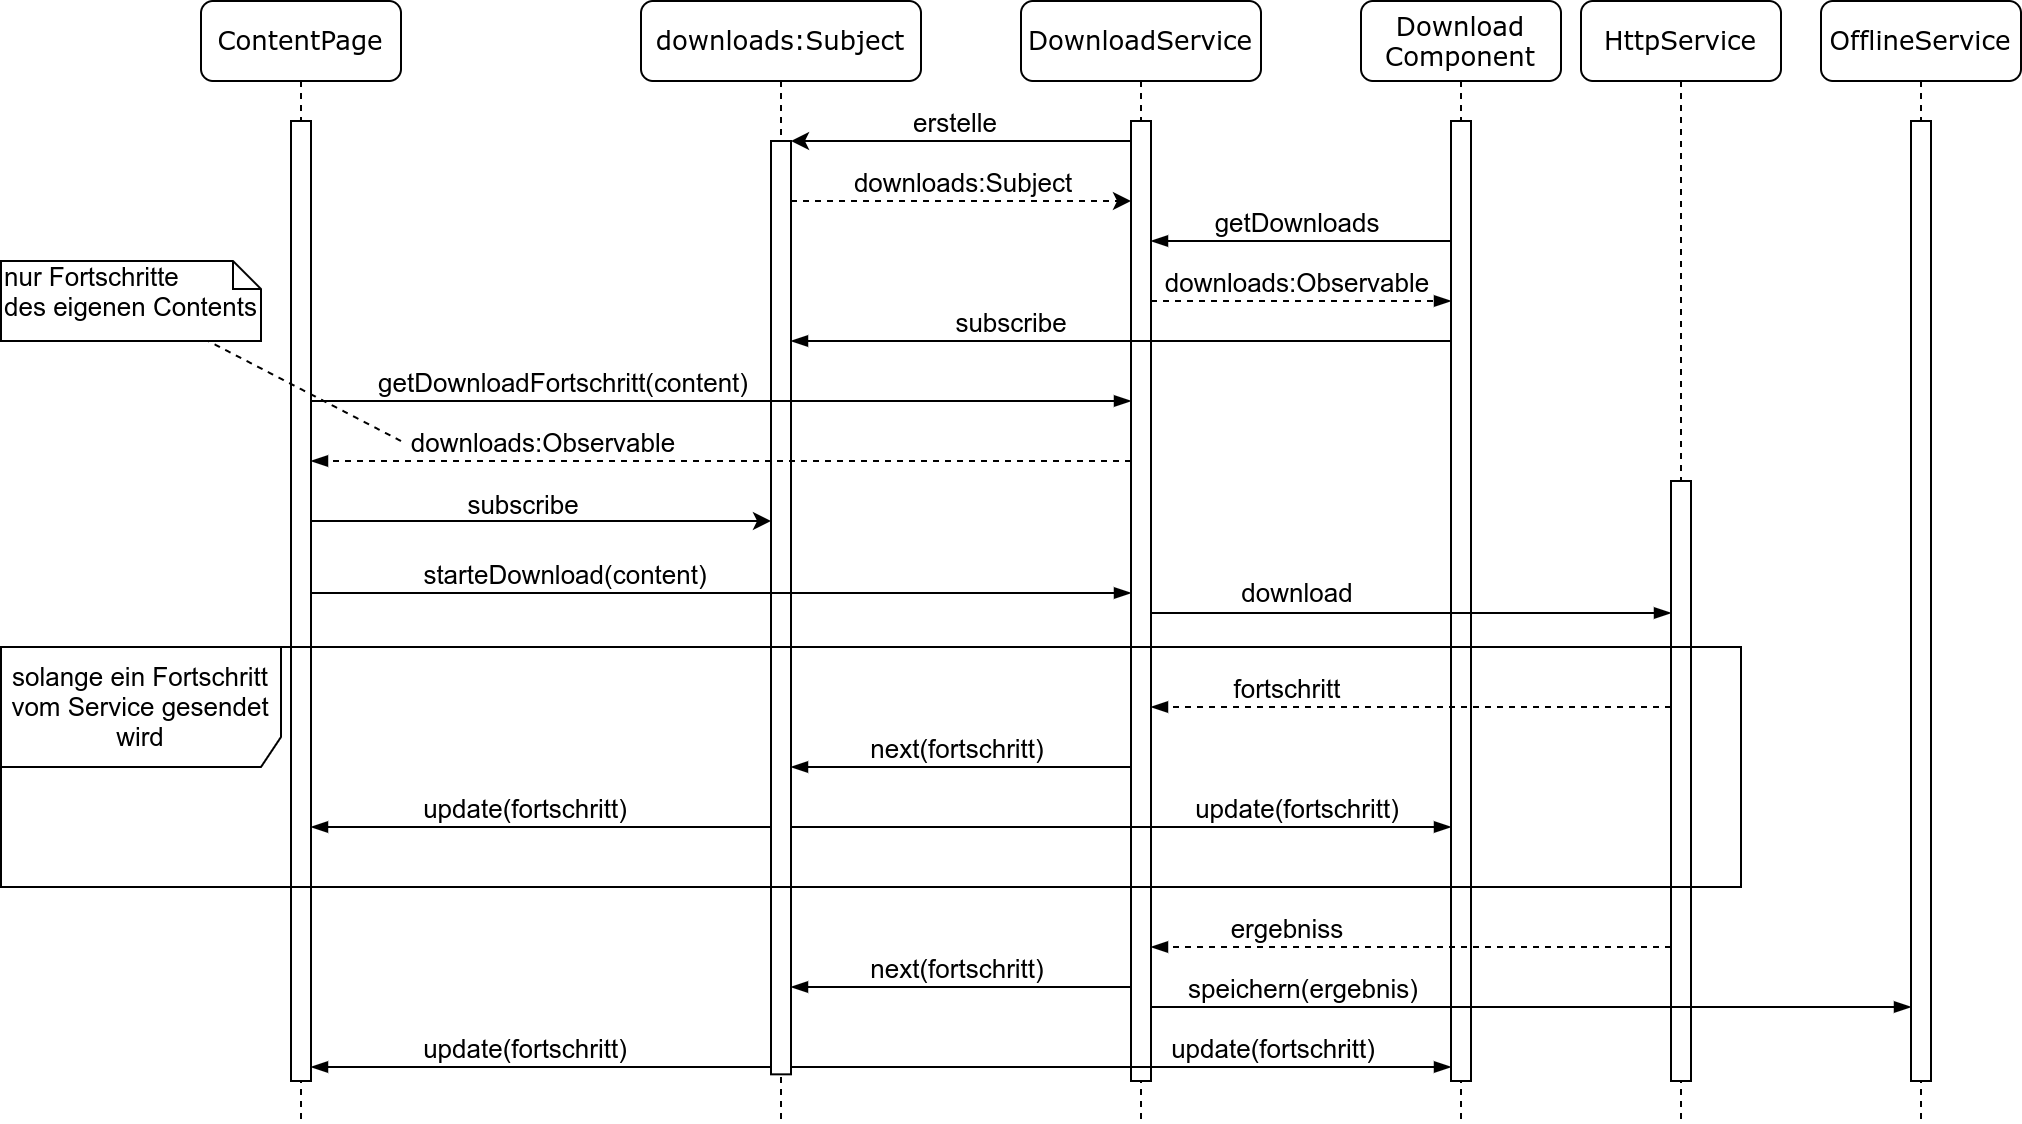
\includegraphics[width=22cm]{diagramme/download-sequenzdiagramm}
  \caption{Sequenzdiagramm für den Download von Dateien}
  \label{diagramme/download-sequenzdiagramm}
\end{sidewaysfigure}

\section{Grafische Oberfläche}
